%This is the third chapter of the dissertation

%The following command starts your chapter. If you want different titles used in your ToC and at the top of the page throughout the chapter, you can specify those values here. Since Columbia doesn't want extra information in the headers and footers, the "Top of Page Title" value won't actually appear.

\pagestyle{cu}
\graphicspath{{./AppendixB/images/}}

\chapter[Characterization of Photomultiplier Tubes with the Cascade Model][Characterization of Photomultiplier Tubes with the Cascade Model]{Characterization of Photomultiplier Tubes with the Cascade Model}
\label{app:pmts}



\section{Motivation}

Photomultiplier tubes (PMTs) are widely used to detect low levels of light in many fields of physics, especially in the field of dark matter detection.  However, despite their ubiquitousness, calibration and characterization of the single photoelectron (SPE) charge response of PMTs remains in a fairly basic state.  PMTs are very complicated devices yet they are often treated with a simple approximation: that the SPE charge response is Gaussian \cite{bellamy1994absolute, dossi2000methods}. While this approximation is satisfactory for specific PMTs within certain voltage ranges, it is far from true in general.  Since the Gaussian distribution is not bounded below by zero, the response function cannot be correct for a SPE and oftentimes, when PMT calibrations are performed with low PMT voltages, the response function will have a large probability of producing a non-physical signal. 

Several alternatives have been proposed to improve upon existing methods for determining the single photoelectron response.  An empirical approach is presented in \citeref{de2010methods} but is only relevant when the height of the PMT output is needed and not the integral of the pulse.  Another widely used model independent approach is presented in \citeref{saldanha2017model}.  The model independent approach provides a simple way to accurately determine the mean and variance of the single photoelectron response function.  In many cases, the mean and variance of the SPE response are  enough since at moderate numbers of photoelectrons the response function converges to a Gaussian described by these parameters.  However, at small numbers of photoelectrons, it is important to account completely for the SPE response shape.  Additionally, the results of the model independent method become more susceptible to bias when the background distribution width is large and the PMT gain is low and it requires a consistent and dedicated background measurement, which is not always possible as was the case for neriX.  Background, in this work, is used to describe all signals that are not induced by the laser or diode, such as noise from the electronics, dark counts, or photoelectrons from light sources other than the laser or diode.

In this appendix, we discuss a more realistic model, henceforth referred to as the \textit{cascade model}, which aims at capturing the actual behavior and mechanics of the PMT.  As with the other major analyses presented in this work(see \secref{sec:xe1t_er_nr_calibration} and \secref{sec:nerix_analysis} for more details on these analyses), the model does not have an analytical form that can be used for parameter estimation but rather relies on running a Monte Carlo (MC) simulation with each set of parameters under test to find the posterior and the best-fit parameters given the data.  These MC simulations also are performed using the GPU framework discussed in \appref{app:gpus}.


\section{The Cascade Single Photoelectron Charge Response Model}
\label{sec:pmt_cascade_description}

With almost countless varieties of PMTs used in different settings, it is impossible to describe a single model that will accurately characterize all PMTs under all circumstances.  However, in this work, we present a SPE response model that has been found to be successful for two very different PMTs and which is physically motivated according to \citeref{carter1980photomultiplier}.  

In the cascade model, there are three different physical processes that can produce an output signal.  Each of these scenarios is depicted in \figref{fig:fig-pmt_diagram}.
\begin{enumerate}
	\item Full amplification: this is the most common process for producing a signal from the PMT.  This occurs when a photon is absorbed by the photocathode which then releases an electron (referred to as a photoelectron).  This electron is then accelerated to the first of the multiple dynodes found inside of the PMT.  This electron will then strike the surface of the dynode and release more electrons in the process.  These secondary electrons are then accelerated towards the second dynode.  This process continues through all the dynode stages and results in a signal that is proportional to the number of photons initially absorbed by the photocathode.
    \item Bad trajectory amplification of photoelectrons from the photocathode: this is very similar to full amplification with a single important change.  The electron released from the photocathode may follow a non-ideal trajectory which will result in secondary electrons potentially not reaching the next stage of amplification.  This will ultimately result in lower amplification and is caused by electric field imperfections in the PMT.  
    \item Amplification from direct excitation of the first dynode: this occurs when a photon passes through the photocathode and strikes the first dynode, in turn releasing an electron.  This electron then follows the chain of amplification, albeit with one less dynode.  The initial electron may also follow a non-ideal trajectory which results in smaller than normal amplification even accounting for the loss of a dynode stage.
\end{enumerate}

\begin{figure}[t]
\centering
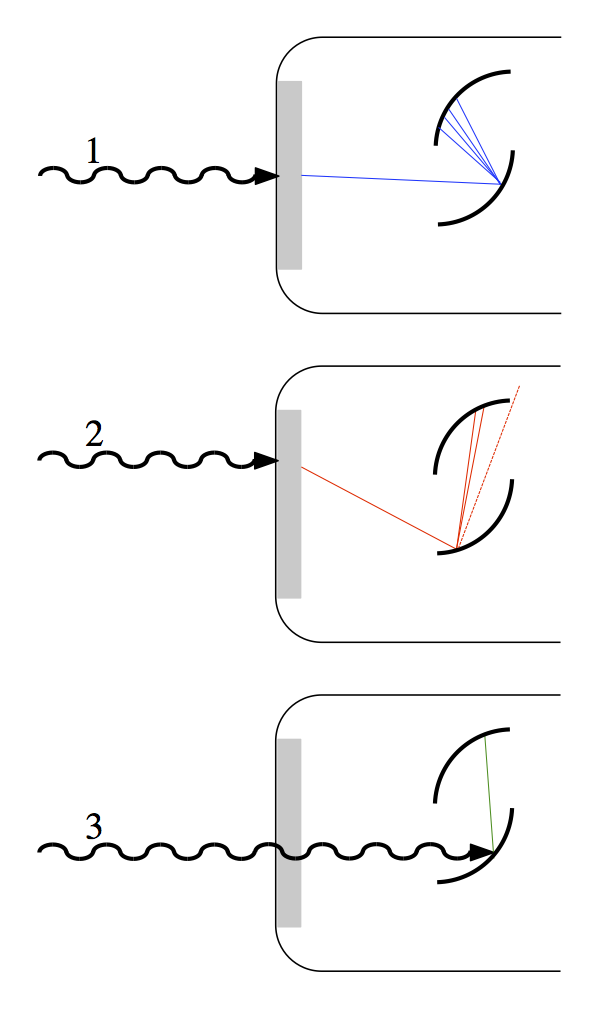
\includegraphics[width=7cm]{final_pmt_diagram_2.png}
\caption{The three possible scenarios for photoelectrons in the cascade model.  Scenario 1 shows the standard full-amplification: a photon is absorbed in the photocathode and an electron is amplified through the dynode chain.  Scenario 2 shows a non-ideal trajectory: a photon is absorbed in the photocathode but the electron follows a slightly different trajectory, due to field imperfections, and suffers a slightly lower amplification.  Scenario 3 shows a photon passing through the photocathode and releasing an electron on the first dynode.  Note that in this scenario  the amplification at each dynode may depend on where the incident photon strikes the first dynode.}
\label{fig:fig-pmt_diagram}
\end{figure}

To approximate these three physical processes in the SPE response, eight parameters were used:

\begin{itemize}
	%\item $\mu_{pi}$: the mean number of photons incident in a given event.
    \item $p_{pc}$: the probability that an incident photon produces a photoelectron from the photocathode that is amplified.
    \item $p_{fd}$: the probability that an incident photon produces a photoelectron from the first dynode that is amplified.  Note that an incident photon cannot create a photoelectron on both the photocathode and the first dynode.
    \item $p_{bt}$: the probability that a photoelectron from the photocathode will follow a non-ideal trajectory through the dynodes and will require a correction to the resulting amplification.
    \item $\mu_{epd}$, $\sigma_{epd}^2$: the mean and variance of the truncated discrete Gaussian, used to find how many secondary electrons are produced by each incoming electron at each dynode stage, for the smallest electric field in the dynode chain.  These parameters are increased linearly with the electric field at each dynode stage.
    \item $p_c$: the probability that secondary electrons escape the surface of the dynode and reach the following dynode.
    \item $c_{fd}$, $c_{bt}$: the corrections applied to $p_c$ accounting for differences in photoelectron amplification from the first dynode and for underamplification due to bad trajectories.
    %\item $\mu_{bkg}$, $\sigma_{bkg}$: the mean and width of the Gaussian background peak.  If an independent, background-only dataset exists, one can constrain these parameters with a prior given by the best fit values and uncertainties for the mean and width of the background Gaussian peak.%: $\hat{\hat{\mu}}_{bkg}$, $\hat{\hat{\sigma}}_{bkg}$, $\sigma_{\hat{\hat{\mu}}_{bkg}}$, and $\sigma_{\hat{\hat{\sigma}}_{bkg}}$.


    
\end{itemize}


The photoelectron of the SPE response in the cascade model has two potential points of origin: (1) the photocathode or (2) the first dynode.  This implies that the origination is described by a binomial process with a single trial.

\begin{equation}
        n_{pc} \sim B\left(n=1; p=\frac{p_{pc}}{p_{pc}+p_{fd}}\right), \qquad
        n_{fd} = 1 - n_{pc}.
\end{equation}

In the above equation, $n_{pc}$ accounts for all electrons coming from the photocathode and $n_{fd}$ accounts for all electrons coming directly from the first dynode.


It is important to note that certain PMTs are found to produce two photoelectrons instead of a single photoelectron at the photocathode with a measured probability, $p_{DPE}$, at certain wavelengths of incident light.  A measurement of this effect is described in \citeref{faham2015measurements}.  One can simply account for this double photoelectron effect by adding a binomial process.

\begin{equation}
        n_{pc} \leftarrow n_{pc} + B(n=n_{pc}, p=p_{DPE}).
\end{equation}

Further dividing electrons from the photocathode, the model assumes a fixed probability that the electron will follow a bad trajectory.


\begin{equation}
n_{bt} \sim B(n=n_{pc}, p=p_{bt}), \qquad
n_{fa} = n_{pc} - n_{bt}.
\end{equation}

In the above equation, $n_{bt}$ is the number of electrons from the photocathode that follow a bad trajectory, resulting in underamplification, and $n_{fa}$ is the number of electrons that are fully amplified from the photocathode through the entire dynode chain.

%Fig. \ref{fig:fig-pmt_diagram} shows a diagram for each of these three scenarios for a photon that creates an electron.

With all three potential signal sources accounted for, one can now consider the dynode chain.  For the dynode chain, it is assumed that the electrons follow a Galton-Watson branching process as described in \citeref{tan1982statistical}.  However, instead of the Poisson distribution as described in \citeref{tan1982statistical}, the model assumes that the the number of secondary electrons at each dynode stage is described by a discrete Gaussian (as described in \citeref{dwarakanath2014sampling}) and a binomial process (with probability of success $p_c$) to be as general as possible (since the shape and variance of a Poisson distribution are fixed by its mean).  This iterative process is described in \eqnref{gw_1} and \eqnref{gw_2}.  In these equations, $h_{i}$ is the number of secondary electrons leaving the $i^{th}$ dynode while $m_{i}$ is the number of electrons that reach the $i^{th}$ dynode.

\begin{equation}
\label{gw_1}
h_{i} \sim DG(n=m_{i} \mu_{epd}, \sigma^2 = m_{i} \sigma^2_{epd}).
\end{equation}
\begin{equation}
\label{gw_2}
m_{i+1} \sim B(n=h_{i}, p=p_{c}).
\end{equation}

For the bad trajectory electrons from the photocathode and the electrons from the direct excitation of the first dynode, the Galton-Watson process is modified such that $p_{c} \rightarrow p_{c} c_{fd}$ or $p_{c} \rightarrow p_{c} c_{bt}$ to account for their non-ideal trajectory.  This correction is applied identically to each dynode in the chain.  Differences in the electric fields between dynodes are accounted for by proportionally increasing the mean and variance of the discrete Gaussian ($\mu_{epd}$ and $\sigma^2_{epd}$ represent the mean and variance of the Galton-Watson process for the smallest electric field in the chain).

While there is not an analytical function to describe the SPE response in the cascade model, we can use the procedure outlined in \appref{app:gpus} to define a likelihood and ultimately sample the posterior.


\section{Data Collection}


Low light level data was used from two independent experiments using two different methods of data collection and PMTs.  The first set of data was provided by the experiment described in \citeref{saldanha2017model}.  This data is from a Hamamatsu R11410, a 3 inch PMT, the low-background version of which was used in the XENON1T experiment \cite{aprile2016physics}. The PMT was operated in a dark box with a 405 nm pulsed laser behind a filter with an attenuation factor $\eta$.  By changing $\eta$, one can change the mean number of incident photons.  Background measurements were also taken for this data in the exact same operating conditions except with the laser light blocked.

The second set of data is from the neriX detector discussed in chapter four.  This data is from a Hamamatsu R6041-406 SEL 2'' PMT in LXe illuminated by a blue pulsed LED located inside the detector.  The PMT used to collect this data operates at a significantly lower gain than the PMT used in \citeref{saldanha2017model} and has worse noise conditions.  Also, identical conditions during background measurements could not be guaranteed and therefore the model independent approach could not be used to characterize this PMT.

In both experiments, the digitized waveforms were integrated with consistent acquisition windows.

Also, the light used to illuminate the PMTs in both experiments had a wavelength larger than 400 nm so double photoelectron emission (DPE) effects were not included \cite{faham2015measurements}.  As mentioned in \secref{sec:pmt_cascade_description}, DPE effects can straight-forwardly be added to the cascade model if needed.


\section{Results}

\subsection{Response Characterizations}

Three methods were used to characterize the PMTs for which data was collected.  The first was the cascade model, for which the SPE response was described in detail in \secref{sec:pmt_cascade_description}.  With the model of the SPE response, we can approximate the response of larger signals by convolving the SPE response function ($f_1$ in \eqnref{spe_convolution}) with itself for the number of photoelectrons needed.  Finally, one must consider detector specific effects by convolving the signal with the background spectrum ($f_0$ as defined in \eqnref{bkg_spec}).  In this work, the background is approximated as Gaussian from independent measurements.

\begin{equation}
        \label{bkg_spec}
        f_0(x) = N(\mu=\mu_{bkg}, \sigma^2=\sigma^2_{bkg}).
\end{equation}
\begin{equation}
        \label{spe_convolution}
        f_n(x) = f_0(x) \circledast \overbrace{f_1(x) \circledast f_1(x) \circledast \ldots \circledast f_1(x)}^{\text{n times}}.
\end{equation}

To perform parameter estimation, one must consider how the PMT is illuminated.  Since low light levels are used, one expects the number of photoelectrons produced per light pulse to follow a Poisson distribution with a mean $\lambda$.  One then combines the individual contributions to define the PDF of the full spectrum at a certain light level that will be used (\eqnref{cascade_fit_full}).

\begin{equation}
        \label{cascade_fit_full}
        f(x) = P(k=0, \mu=\lambda) \cdot f_0(x) + \sum^{\infty}_{i=1} (P(k=i, \mu=\lambda) \cdot f_i(x)).
\end{equation}

The second method used was the model independent characterization, which is described in detail in \citeref{saldanha2017model}.  The model independent method uses the statistical properties of the laser calibration charge spectra and a background-only charge spectra to estimate the mean and variance of the single photoelectron response, as well as the mean number of photoelectrons produced per light pulse. This method has the advantage that it does not assume any specific functional form for the SPE response as the PMT response converges to a Gaussian for signals with more than roughly five to ten photoelectrons. However the method requires a dedicated background measurement in identical operating conditions, and additional parameters may be needed if one needs to simulate the full functional response of a PMT at very low light levels.

The third method used to characterize the PMTs was the Gaussian approximation with an underamplified peak.  In this case, the SPE response is the sum of two  Gaussians - one representing fully-amplified photoelectrons and the other representing underamplified photoelectrons.  One can estimate larger signals in the same way as the cascade model: by convolving the SPE response function ($s_1$ as defined in \eqnref{gaussian_spe}) with itself for the number of photoelectrons needed and then with the background as shown in \eqnref{gaussian_mpe}.  


\begin{equation}
        \label{gaussian_spe}
        s_1(x) = N(\mu=\mu_1, \sigma^2=\sigma^2_1) + w \cdot N(\mu=\mu_u, \sigma^2=\sigma^2_u), \, 0 \leq w \leq 1.
\end{equation}
\begin{equation}
        \label{gaussian_mpe}
        g_n(x) = f_0(x) \circledast \overbrace{s_1(x) \circledast s_1(x) \circledast \ldots \circledast s_1(x)}^{\text{n times}}.
\end{equation}

Finally, to produce the PDF for parameter estimation, one defines a mean number of photoelectrons per pulse and sums each peaks individual contributions weighted by a Poisson distribution (\eqnref{eqn:gaussian_pdf}).  This is done in the same way as the cascade model.

\begin{equation}
        \label{eqn:gaussian_pdf}
        g(x) = P(k=0, \mu=\lambda) \cdot f_0(x) + \sum^{\infty}_{i=1} (P(k=i, \mu=\lambda) \cdot g_i(x)).
\end{equation}

In these equations, $\lambda$ is the mean number of PE and $\mu_u$ and $\sigma_u$ are the mean and standard deviation of the underamplified peak.  The Gaussian model is motivated by the work in \citeref{mayani_thesis}.  



\subsection{Hamamatsu R11410 Analysis}

The R11410 data includes a dedicated background measurement that can be used to constrain the model.  For example, an exponential contribution to the background (as suggested in \citeref{bellamy1994absolute}) is ruled out and $\mu_{bkg}$ and $\sigma_{bkg}$ are constrained with a prior during the fits for both the cascade and Gaussian model (the background spectrum is shown figures 4, 6, and 7 in \citeref{saldanha2017model}).

While in a standard experiment one could take multiple datasets while varying light levels and fit all data simultaneously to calibrate the SPE response, in this work it was decided to fit each light level individually in order to compare these results directly to the model independent method and the Gaussian model.  

The results of the fit are shown in \tabref{tab-1}.  In the table, $\eta$ is the attenuation factor of the filter in between the laser and PMT, $\lambda$ is the mean number of photoelectrons per light pulse, and $\mu$ and $\sigma$ are the mean and standard deviation of the resulting SPE response function.  All uncertainties shown are statistical.  Note that the model independent (MI) results and the cascade model (CM) results agree typically within a few percent and never disagree by more than 10\%.



\begin{table*}[t]
%\fontsize{4.9}{8}
%\selectfont
\centering

\def\arraystretch{1.2}
\resizebox{\textwidth}{!}{
\begin{tabular}{cc|ccccc}


\multicolumn{2}{c|}{Voltage [V]} & 1400 & 1500 & 1600 & 1700 & 1700 \\

\multicolumn{2}{c|}{$\eta$} & 2E5 & 2E5 & 2E5 & 2E5 & 1E5 \\ \hline

\multirow{3}{*}{$\lambda$} & MI & $1.257 \pm 0.005$ & $1.289 \pm 0.005$ & $1.324 \pm 0.005$ & $1.351 \pm 0.005$ & $2.395 \pm 0.008$ \\
						   & CM & $1.226^{+0.123}_{-0.043}$ & $1.256^{+0.010}_{-0.010}$ & $1.300^{+0.009}_{-0.008}$ & $1.315^{+0.008}_{-0.009}$ & $2.372^{+0.025}_{-0.022}$ \\
						   & GM & $1.188^{+0.022}_{-0.018}$ & $1.201^{+0.009}_{-0.008}$ & $1.234^{+0.011}_{-0.009}$ & $1.275^{+0.014}_{-0.013}$ & $2.284^{+0.029}_{-0.032}$ \\ \hline

$\lambda_{FA}$ & CM & $1.063^{+0.007}_{-0.007}$ & $1.039^{+0.007}_{-0.007}$ & $1.039^{+0.006}_{-0.006}$ & $1.042^{+0.006}_{-0.006}$ & $1.842^{+0.015}_{-0.016}$ \\ \hline

\multirow{3}{*}{$\mu$ [$\textrm{e}^-$]} & MI & $1.88\textrm{E}6 \pm 7\textrm{E}3$ & $3.10\textrm{E}6 \pm 1\textrm{E}4$ & $4.98\textrm{E}6 \pm 2\textrm{E}4$ & $7.88\textrm{E}6 \pm 2\textrm{E}4$ & $7.90\textrm{E}6 \pm 2\textrm{E}4$ \\
                       & CM & $1.87\textrm{\textrm{E}}6 \pm 1.5\textrm{E}5$ & $3.17\textrm{E}6 \pm 2\textrm{E}4$ & $5.12\textrm{E}6 \pm 3\textrm{E}4$ & $8.03\textrm{E}6 \pm 4\textrm{E}4$ & $7.88\textrm{E}6 \pm 8\textrm{E}4$ \\
                       & GM & $1.96\textrm{E}6 \pm 3\textrm{E}4$ & $3.30\textrm{E}6 \pm 2\textrm{E}4$ & $5.34\textrm{E}6 \pm 5\textrm{E}4$ & $8.19\textrm{E}6 \pm 9\textrm{E}4$ & $8.08\textrm{E}6 \pm 7\textrm{E}4$ \\ \hline
                       
\multirow{3}{*}{$\sigma$ [$\textrm{e}^-$]} & MI & $8.64\textrm{E}5 \pm 1\textrm{E}4$ & $1.56\textrm{E}6 \pm 2\textrm{E}4$ & $2.84\textrm{E}6 \pm 2\textrm{E}4$ & $4.49\textrm{E}6 \pm 5\textrm{E}4$ & $4.51\textrm{E}6 \pm 5\textrm{E}4$ \\
                       & CM & $9.05\textrm{E}5 \pm 9\textrm{E}4$ & $1.56\textrm{E}6 \pm 1\textrm{E}4$ & $2.66\textrm{E}6 \pm 2\textrm{E}4$ & $4.26\textrm{E}6 \pm 3\textrm{E}4$ & $4.34\textrm{E}6 \pm 5\textrm{E}4$ \\
                       & GM & $7.73\textrm{E}5 \pm 3\textrm{E}4$ & $1.38\textrm{E}6 \pm 2\textrm{E}4$ & $2.35\textrm{E}6 \pm 2\textrm{E}4$ & $3.80\textrm{E}6 \pm 3\textrm{E}4$ & $3.81\textrm{E}6 \pm 3\textrm{E}4$ \\ \hline
                       
\multicolumn{2}{c|}{$ln \left( \frac{\mathcal{L}_{CM}}{\mathcal{L}_{GM}} \right)$} & -14.5 & 17.2 & 257.4 & 567.2 & 183.8 \\



\end{tabular}
}
\caption{Comparison of model independent (MI), cascade model (CM), and Gaussian model (GM) using the R11410 PMT.}
\label{tab-1}
\end{table*}



Also of note in \tabref{tab-1} is the row $\lambda_{FA}$ denoting the mean number of photoelectrons fully amplified.  Unlike the other $\lambda$ measurements, $\lambda_{FA}$ should be approximately voltage independent since underamplification effects are removed.  As can be seen, all $\lambda_{FA}$ with the same attenuation $\eta$ agree within $\sim$1\%, providing a cross-check on the cascade model fit.

Another very important feature of the table is the last row, which compares the best-fit log-likelihood of the cascade model to the best-fit log-likelihood of the Gaussian model.  The cascade model significantly outperformed the Gaussian model in four out of five of the datasets.  Unsurprisingly, the dataset where the Gaussian model outperforms the cascade model is when the voltage is lowest and the valley in between the background and single photoelectron peak plays the smallest role in the fit.  This improvement is likely due to the increased freedom in the Gaussian model since the underamplfied peak is almost entirely independent of the fully-amplified peak.




\begin{figure}[p]
        \centering
    
        \subfloat[R11410 PMT at 1400 V with attenuation of 2E5]{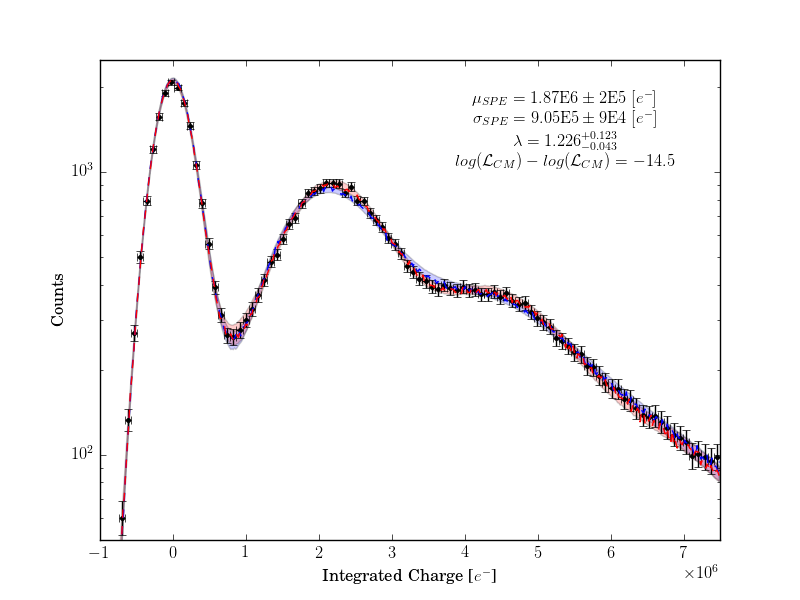
\includegraphics[width=0.48\textwidth]{0067_0068_best_fit}} \hfill
	\subfloat[R11410 PMT at 1500 V with attenuation of 2E5]{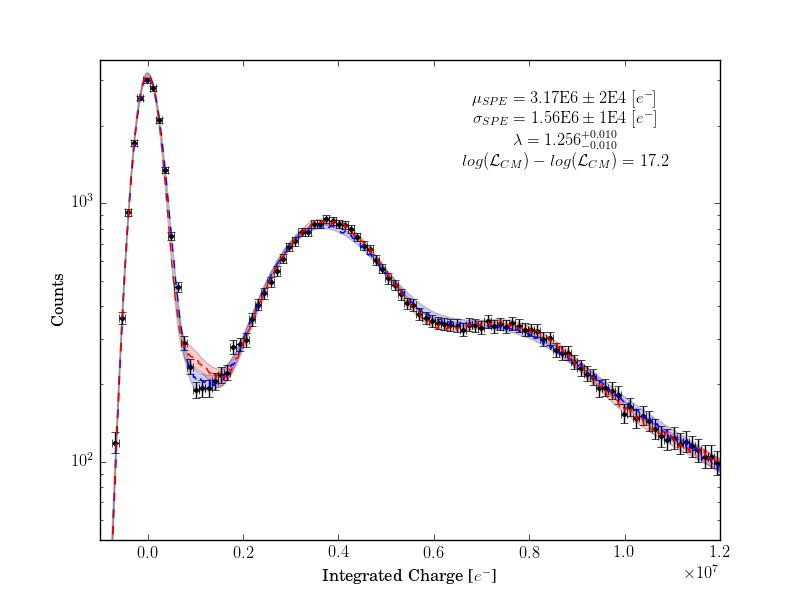
\includegraphics[width=0.48\textwidth]{0066_0065_best_fit}}

        %\vspace{0.5cm}
    

        \subfloat[R11410 PMT at 1600 V with attenuation of 2E5]{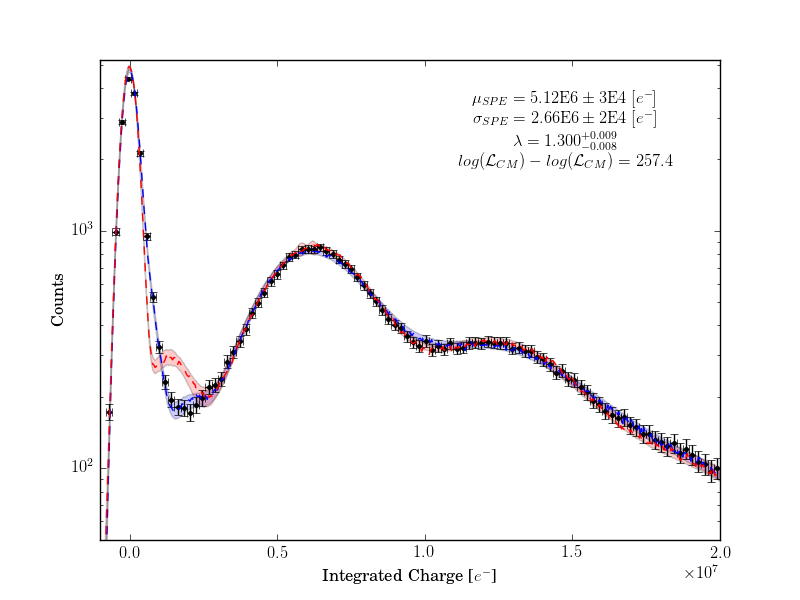
\includegraphics[width=0.48\textwidth]{0062_0061_best_fit}} \hfill
	\subfloat[R11410 PMT at 1700 V with attenuation of 2E5]{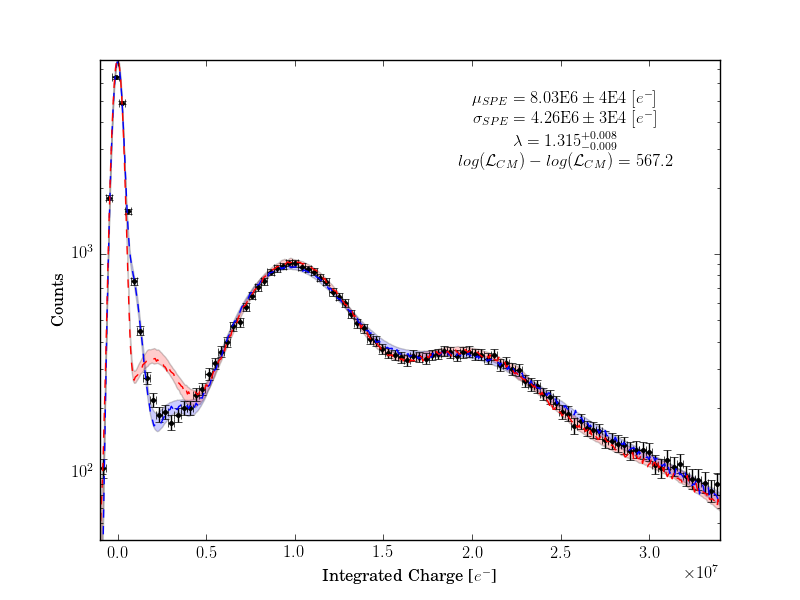
\includegraphics[width=0.48\textwidth]{0071_0072_best_fit}}


	%\vspace{0.5cm}

        \subfloat[R11410 PMT at 1700 V with attenuation of 1E5]{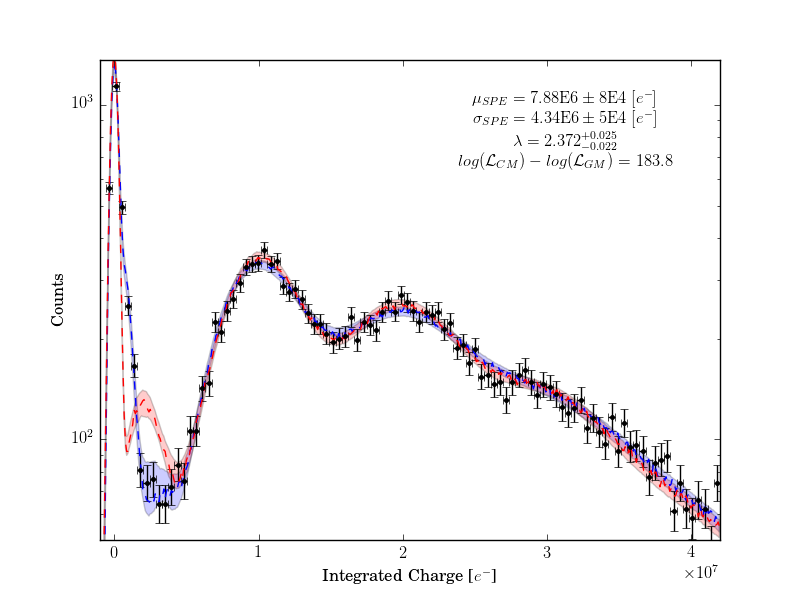
\includegraphics[width=0.48\textwidth]{0073_0074_best_fit}}


        \caption{The laser calibration charge spectra for the R11410 PMT at different voltages and attenuation levels with the best-fit models and 95\% credible regions overlaid.  The cascade model is shown in blue while the Gaussian model is shown in red.  The statistics shown are for the cascade model.}
    
        \label{fig:uc_best_fits}
\end{figure}


\figref{fig:uc_best_fits} shows the best-fits for both the cascade model (blue) and the Gaussian model (red) compared to laser calibration charge data along with the 95\% credible regions of each fit.  Notice that as the gain increases, the Gaussian model is unable to explain the behavior in the valley while the cascade model predicts this behavior well in all five spectra.

% removed from previous paragraph
% The two-sigma credible region is created by making random draws from the posterior of the fit and determining the 95\% confidence interval for a given bin.  

%\begin{figure}[t]
%\centering
%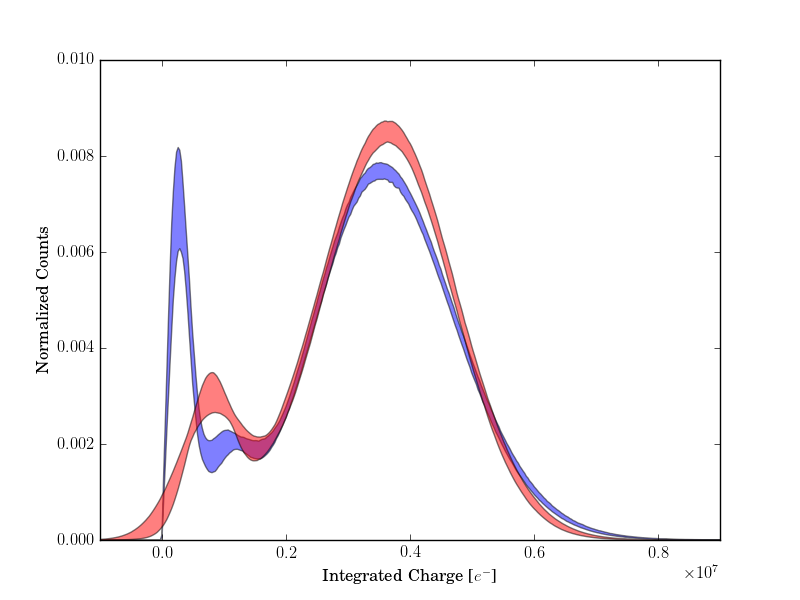
\includegraphics[width=9cm]{uc_spe_response.png}
%\caption{The predicted SPE charge response for the R11410 PMT at 1500 V.  From left to right, one can see the three major features: the underamplified peak from photons striking the first dynode, the underamplified peak from a non-ideal trajectory, and the fully-amplified peak.}
%\label{fig:fig-2}
%\end{figure}


\begin{figure}[t]
\centering
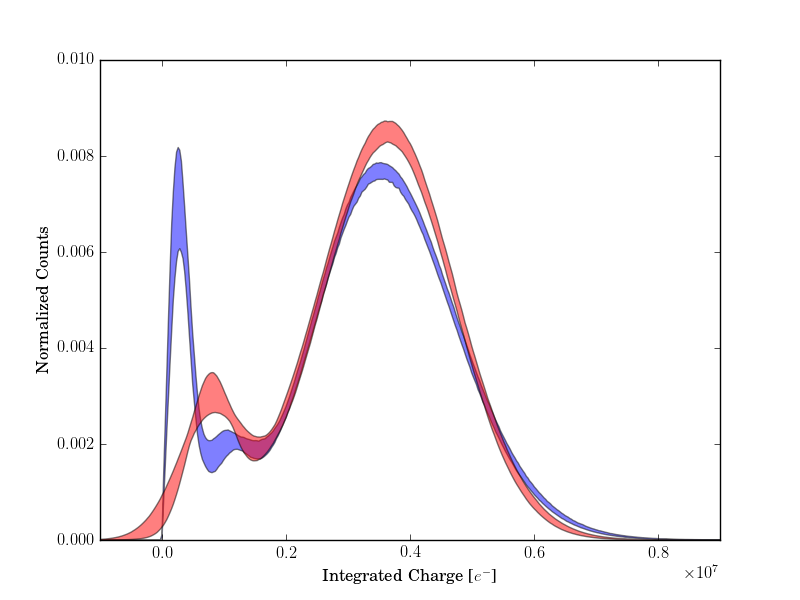
\includegraphics[width=9cm]{uc_spe_response.png}
\caption{The predicted SPE charge response for the R11410 PMT at 1500 V for the cascade model (blue) and the Gaussian model (red).  In the cascade model SPE charge response spectrum one can see, from left to right, the three major features: the underamplified peak from photons striking the first dynode, the underamplified peak from a non-ideal trajectory for electrons from the photocathode, and the fully-amplified peak.  At such a high gain the fully-amplified peak (right-most) of the cascade and Gaussian models agree.  However, there is a large discrepancy in the region of underamplified electrons.}
\label{fig:fig-2}
\end{figure}




In \figref{fig:fig-2} one can see the predicted SPE charge response for the R11410 PMT at 1500 V without background convolution.  The region shown is again the 95\% confidence interval.  One can see the three major features going from left to right: the underamplified peak from photons striking the first dynode, the underamplified peak from a non-ideal trajectory, and the fully-amplified peak.  Note that the signal can naturally never be less than zero unlike most analytical models that are either truncated or allowed to extend into a non-physical region.  The fully-amplified signal (right-most peak) is fairly symmetric - this is because this PMT operates at high gain and has good resolution.  This, however, will not be the case when looking at the fully-amplified peak for the R6041-406 PMT in \secref{sec:pmt_nerix_analysis}.




\begin{table}
\centering

\begin{tabular}{|c|c|c|c|c|}
\hline
Voltage {[}V{]} & $\eta$ & Reduced $\chi^2$ & $p_{\chi^2}$ & $p_{KS}$  \\ \hline
1400 & 2E5 & 0.67 & 0.991 & 0.274 \\ \hline
1500 & 2E5 & 0.95 & 0.604 & 0.259 \\ \hline
1600 & 2E5 & 0.90 & 0.742 & 0.287 \\ \hline
1700 & 2E5 & 1.28 & 0.037 & 0.327 \\ \hline
1700 & 1E5 & 0.98 & 0.539 & 0.279 \\ \hline

\end{tabular}
\caption{Goodness of Fit Tests For R11410 with Cascade Model.}
\label{tab-gof}

\end{table}

Shown in \tabref{tab-gof} are the results of the goodness of fit tests for the best-fit parameters.  Since the parameter estimation is performed in a single dimension, one can look at the relatively simple $\chi^2$ test and the more robust Kolmogorov-Smirnov (KS) test.  While there is more fluctuation from the $\chi^2$ test, all tests show little or no evidence against the cascade model.





\subsection{Hamamatsu R6041-406 Analysis}
\label{sec:pmt_nerix_analysis}

\begin{table*}[t]
%\fontsize{4.9}{8}
%\selectfont
\centering

\def\arraystretch{1.2}
\begin{tabular}{cc|cc}


\multicolumn{2}{c|}{Voltage [V]} & 800 & 800 \\

\multicolumn{2}{c|}{Light Level} & \RNum{1} & \RNum{2} \\ \hline

\multirow{2}{*}{$\lambda$} & CM & $1.237^{+0.070}_{-0.042}$ & $2.455^{+0.148}_{-0.140}$ \\
						   & GM & $1.403^{+0.064}_{-0.046}$ & $2.709^{+0.108}_{-0.098}$ \\ \hline

\multirow{2}{*}{$\mu$ [$\textrm{e}^-$]} & CM & $8.43\textrm{E}5 \pm 4.8\textrm{E}4$ & $8.53\textrm{E}5 \pm 6.8\textrm{E}4$ \\
                       & GM & $7.57\textrm{E}5 \pm 3.2\textrm{E}4$ & $7.50\textrm{E}5 \pm 2.3\textrm{E}4$ \\ \hline
                       
\multirow{2}{*}{$\sigma$ [$\textrm{e}^-$]} & CM & $5.61\textrm{E}5 \pm 1.7\textrm{E}4$ & $5.89\textrm{E}5 \pm 1.7\textrm{E}4$ \\
                          & GM & $5.79\textrm{E}5 \pm 1.1\textrm{E}4$ & $6.00\textrm{E}5 \pm 1.2\textrm{E}4$ \\ \hline
                       
\multicolumn{2}{c|}{$ln \left( \frac{\mathcal{L}_{CM}}{\mathcal{L}_{GM}} \right)$} & 4.9 & 11.9 \\


\end{tabular}
\caption{Comparison of cascade and Gaussian models using the R6041-406 PMT.}
\label{tab-nerix}

\end{table*}






\begin{table}[t]
\centering

\begin{tabular}{|c|c|c|c|c|}
\hline
Voltage {[}V{]} & Light Level & Reduced $\chi^2$ & $p_{\chi^2}$ & $p_{KS}$  \\ \hline
800 & I & 1.39 & 0.009 & 0.361 \\ \hline
800 & II & 1.50 & 0.002 & 0.353 \\ \hline

\end{tabular}
\caption{Goodness of Fit Tests For R6041-406 with Cascade Model.}
\label{tab-gof_nerix}

\end{table}




In addition to the analysis performed with a PMT capable of large gains, the cascade model was also used to calibrate a PMT that must operate at significantly lower gains and with worse noise conditions.  While a background measurement was taken, since the calibration is done in situ with an LED and pulser it is impossible to confirm that noise conditions were the same between the dedicated background measurement (pulser off) and the measurements with the pulser on.  For this reason and given that the width of the background peak is on the order of the SPE response, the model independent approach cannot be used.  





Since the dedicated background measurements for this PMT could not be used, one would normally try multiple background models to study the potential systematic effects.  However, in this work, only the Gaussian background model is examined for consistency.

In this specific calibration, two light levels were used which are denoted \RNum{1} and \RNum{2} corresponding to different pulser voltages used in conjunction with a blue LED.  While for the detector discussed in \citeref{goetzke2016measurement} these two light levels were fit simultaneously, only the results from individual fits are shown for consistency.

The results of the parameter estimation and the goodness of fit tests are shown in \tabref{tab-nerix} and \tabref{tab-gof_nerix}.  The best fit and the 95\% credible region for each light level can be found in \figref{fig:nerix_best_fits}.  While the $\chi^2$ test shows evidence against the cascade model, it seems that this is solely due to the behavior in a handful bins that fall outside of the 95\% credible region as seen in both spectra in \figref{fig:nerix_best_fits}.  This hypothesis is further supported by the results of the Kolmogorov-Smirnov test, which shows no evidence against the cascade model.  As a further cross-check, one can also compare the mean and standard deviation of the response function from both light levels which agree with each other well within uncertainty.


\begin{figure}[t]
        \centering
        
        \subfloat[R6041-406 PMT at 800 V at light level I]{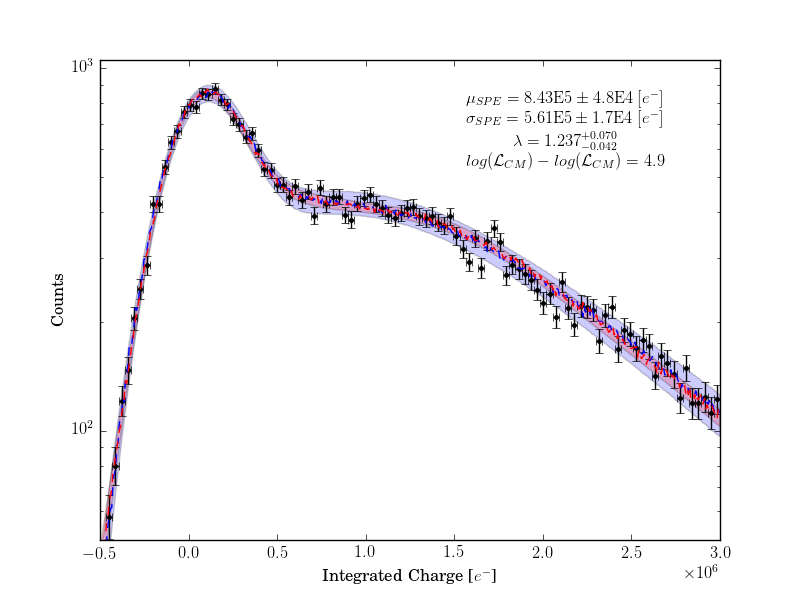
\includegraphics[width=0.48\textwidth]{nerix_160418_1523_best_fit}} \hfill
	\subfloat[R6041-406 PMT at 800 V at light level II]{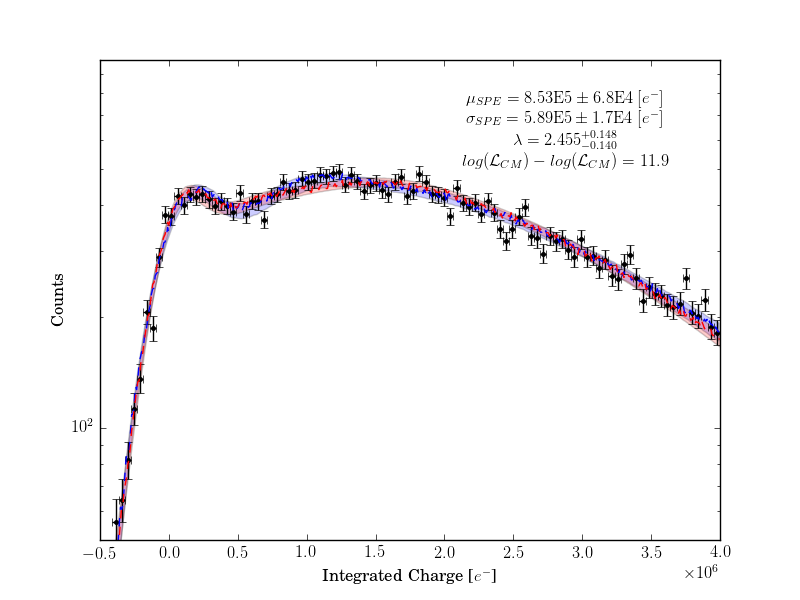
\includegraphics[width=0.48\textwidth]{nerix_160418_1531_best_fit}}
        
        
        \caption{The diode calibration charge spectra for the R6041-406 PMT at 800 V with the best-fit models and 95\% credible regions overlaid.  The cascade model is shown in blue while the Gaussian model is shown in red.  The statistics shown are for the cascade model.}
    
        \label{fig:nerix_best_fits}
\end{figure}



\begin{figure}[t]
\centering
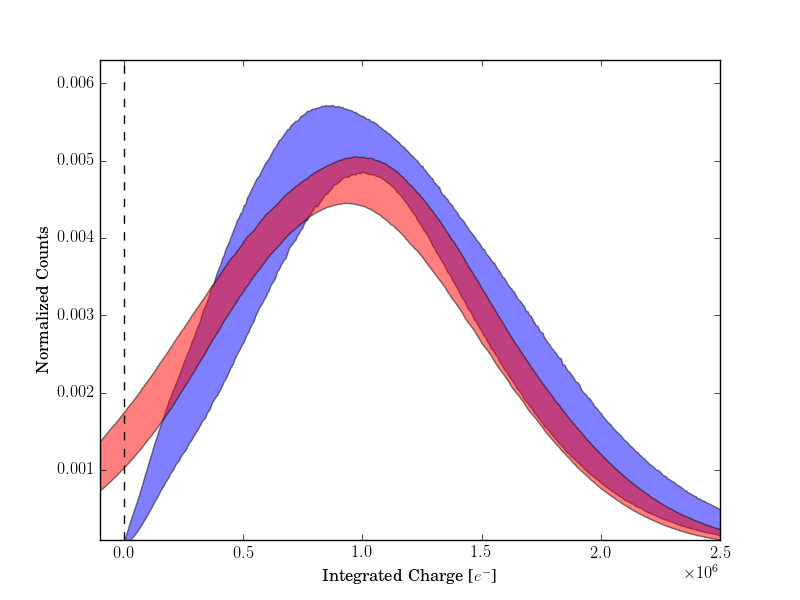
\includegraphics[width=9cm]{nerix_spe_response.png}
\caption{The predicted fully-amplified photoelectron response for the R6041-406 PMT at 800 V.  Notice the asymmetry in the cascade model response (shown in blue) and how far into the unphysical regime the Gaussian model response goes (shown in red). }
\label{fig:fig-nerix_spe}
\end{figure}

While the cascade model outperforms the Gaussian model in fit quality, as seen in the log-likelihood difference, the real power of the cascade model can be seen in \figref{fig:fig-nerix_spe}, which shows the fully-amplified peak only for both models without background convolution.  Notice again that the cascade model naturally begins at zero signal and has the asymmetry that one would expect while the Gaussian model predicts negative signal roughly 15\% of the time from the fully-amplified peak.  Clearly this prediction is not physical and would cause issues in MC simulations of the PMT.



\section{Conclusions}


While the form of the cascade model presented will change for each type of PMT used in a different setting, we have shown that for the PMTs used in these two experiments that the cascade model is a much more realistic approximation of the photomultiplication process, agrees well with data, and is a drastic improvement in almost all cases versus the Gaussian model that is typically used for characterization of photomultipliers.  It is important that in future applications, the analyzer checks different sources of underamplified electrons and different background models if a dedicated background measurement was not performed.  Parameters of the model may be further constrained by estimating them with multiple light levels fit simultaneously.

We recommend that the cascade model be used in conjunction with the model independent prescription described in detail in \citeref{saldanha2017model}.  Since it is relatively unlikely for a PMT's characteristics to change during a measurement, we recommend that an initial characterization be performed using the cascade model and cross-checked with the model independent estimation.  Following the initial characterization, performance can be monitored solely by the model independent estimation with the cascade model reserved for spot checks and diagnosis if PMT performance changes.




